%
% Being an enumeration of various shenanigans.
%

\chapter{Ongoing Events}

% This is true if only doing the flight manual, not the pre-flight
\ifisflight
\putchapterthumb
\fi


% EVENT TEMPLATE

% \subsection*{}
% \begin{description}[leftmargin=6em,noitemsep,style=nextline]
% 	\item[Camp:] 
%   \item[Times:]
% \end{description}

These are events that occur every day of the burn in some way.

\vbox{
\subsection*{BOOTY PRINTS}
\begin{description}[leftmargin=6em,noitemsep,style=nextline]
   \item[Location:] Alcoholic Alliterators
    \item[Host:] AssCommander
\end{description}

All burner butts on deck! This interactive art project turns the Lunatic Lounge into a printshop where you provide a surface (Booty, Boobies, Boots) that we will paint and make art with. Recline in the shade, submit to slathers of paint, leave with a freshly wiped arse or wear your painted flesh around the burn. You can take your prints home to display and say, "YES! What a fine ass I have, What a fine time that was!"

Printshop Provides:: Acrylic \& Tempera Paints, brushes, Paper \& cloth to decorate, Baby wipes to cleanse the canvas. If you want, supplement your experience with something to stamp: A stolen flag? a t-shirt? that camp chair that's about to fall apart?
}

\vbox{
\subsection*{Plant a Flag on the Moon}
\begin{description}[leftmargin=6em,noitemsep,style=nextline]
   \item[Location:] Department of Synergy
\end{description}

Join a game of scavenger hunt/geocaching! We have hidden multiple planets around To The Moon! Can you bring one flag from each planet back to the moon at Department of Synergy? Enter your successful explorations in our Space Travel Logbook!

}

\vbox{
\subsection*{Softkore-aoke}
\begin{description}[leftmargin=6em,noitemsep,style=nextline]
   \item[Location:] Headroom
    \item[Host:] Sarah Anderson
    \item[Start time:] Come by and sign up well let you know :)
\end{description}

Burn version of karaoke

}

\vbox{
\subsection*{Damsel in Dis Dress: Ye Olde Costume Shoppe}
\begin{description}[leftmargin=6em,noitemsep,style=nextline]
   \item[Location:] The Broken Drum
\end{description}

People can come by all weekend and hang up their donations, or browse for some costumery in need of a loving new home.

}

\vbox{
\subsection*{Sound Scapes \& Healing}
\begin{description}[leftmargin=6em,noitemsep,style=nextline]
   \item[Location:] Lucid Lounge on plateau. 
    \item[Start time:] TBD
\end{description}

We host group Sound Meditation Sessions in our dome with signup required to keep it manageable. We encourage participants to leave the world behind and dive into the sonic seas with our gongs and singing bowls to float into a blissful state conducive to a full mental reset, encourage opening of not just heart but also root chakra, and inspire to seek bliss within.  

Nothing needed but an open mind and heart. 
}

\ifisporto
\else
    \vspace*{\fill}
    \begin{figure}[!h]
    \centering
    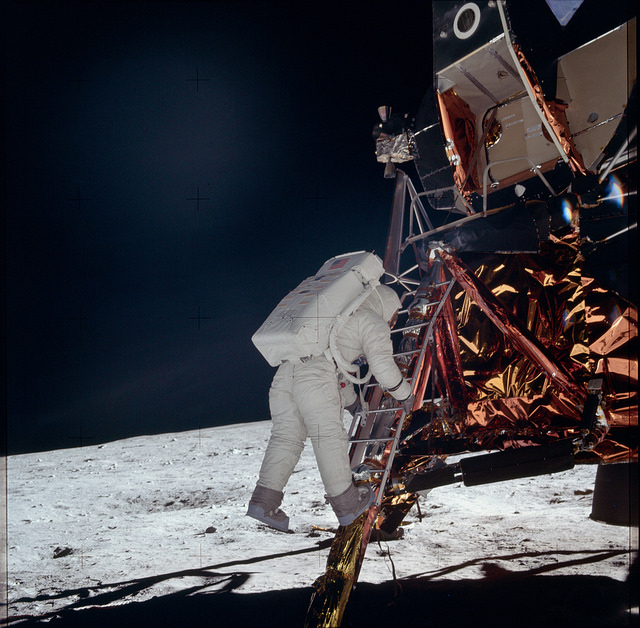
\includegraphics[width=.8\textwidth]{images/arrival.jpg}
    \end{figure}
\fi



\chapter[Thursday]{Thursday Events}

% This is true if only doing the flight manual, not the pre-flight
\ifisflight
\putchapterthumb
\fi


\vbox{
\subsection*{Morning Yoga }
\begin{description}[leftmargin=6em,noitemsep,style=nextline]
   \item[Location:] Acrodesiac Lunartics
    \item[Start time:] 9:00 AM
\end{description}

Gentle yoga flow, all levels. Come stretch and move in our beautiful, shaded studio! 

Bring a mat if you have one, if not, we have extras!
}

\vbox{
\subsection*{Sensual four hand massage}
\begin{description}[leftmargin=6em,noitemsep,style=nextline]
   \item[Location:] Herhisensua
    \item[Time:] 11:00 AM -- 4:00 PM
\end{description}

Sensual massage 

}


\ifisporto
\else
    \vspace*{\fill}
    \begin{figure}[!h]
    \centering
    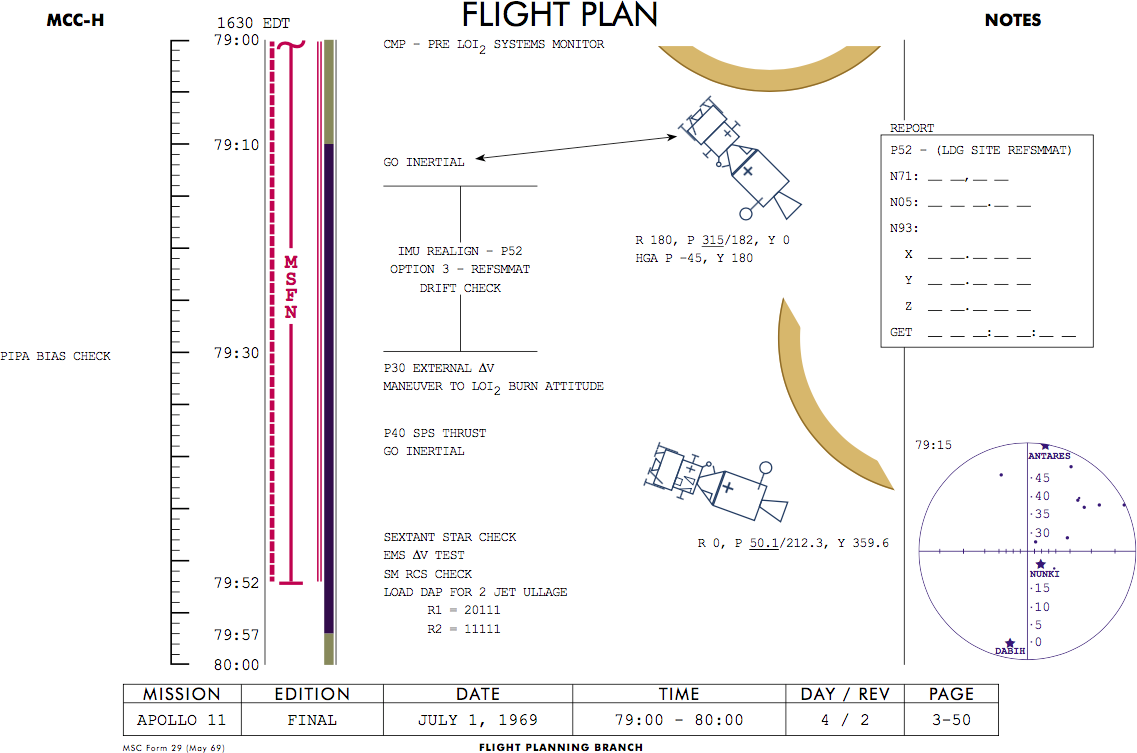
\includegraphics[width=\textwidth]{images/flightplan1.png}
    \end{figure}
    
    \vspace*{\fill}
    \begin{figure}[!h]
    \centering
    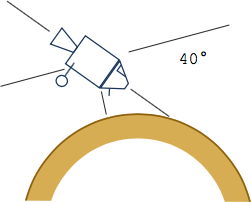
\includegraphics[width=\textwidth]{images/landing2.png}
    \end{figure}
\fi

\vbox{
\subsection*{Axis Mundi Workshop // Climbing the Cosmic Ladder: A Conversation}
\begin{description}[leftmargin=6em,noitemsep,style=nextline]
   \item[Location:] Axis Mundi
    \item[Time:] 3:30 PM -- 4:30 PM
\end{description}

Axis Mundi is known as the hub or axis of the universe, interpreted by many cultures in a wide spectrum of ways. However, the central theme among the sacred symbols is the connection of the underworld, the Earth, and the sky – a dichotomy of integration (oneness) and distance (separate-ness). The roots run deep between theology, culture, and the understanding the universe (which we now call cosmology). Has the universe come into existence a finite time ago? How did it come to be? Will it come to an end? Why are the cosmic evolution and the laws of nature of such a kind that they permit intelligent life to exist? Ancient questions like these have weighed heavy on the curious minds before us, and many still to this day. With some basic concepts and an open mind, we can begin to make sense of the role that the universe itself has played in humanity’s spiritual pursuit of self-actualization. Take an afternoon journey into the cosmos with your astral guide, Minx! 

3:30-4:30pm (adjustable on time – anytime from 1:30-4:30)
}

\ifisporto
\else
    \vspace*{\fill}
    \begin{figure}[!h]
    \centering
    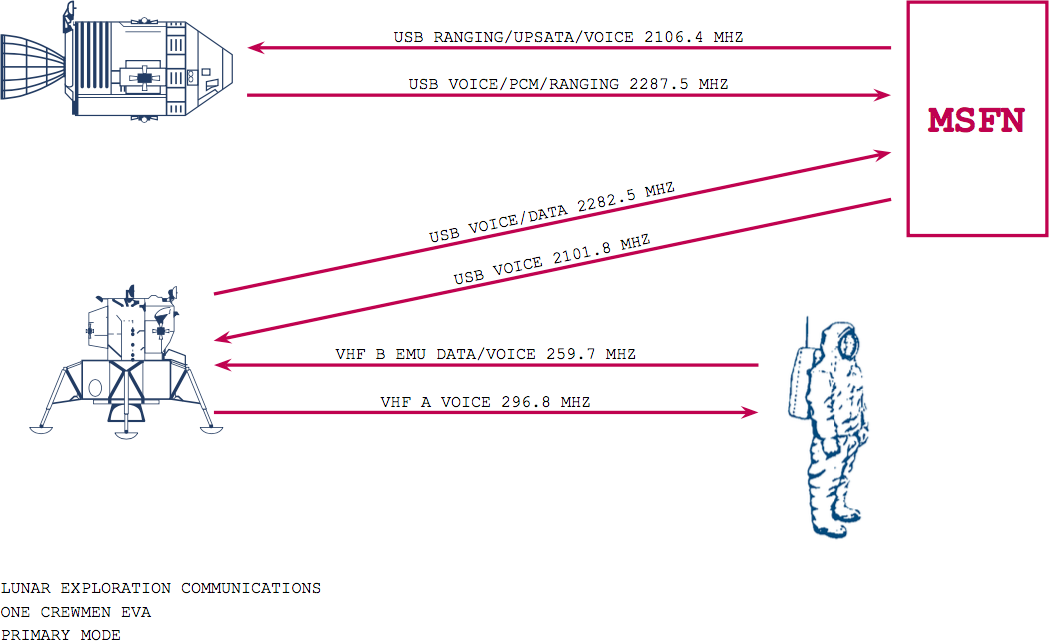
\includegraphics[width=\textwidth]{images/communication2.png}
    \end{figure}
\fi


\vbox{
\subsection*{Dress the LUNARTICS}
\begin{description}[leftmargin=6em,noitemsep,style=nextline]
   \item[Location:] The Tilted Hanger
    \item[Time:] 5:00 PM -- 10:00 PM
\end{description}

Tilted Hanger invites all (radical inclusion) to engage (participate) in (radical self expression) in finding your true burner self! We believe it is our duty (civic responsibility) to guide you in your freedom to receive without a price (de-commodified), receive without having to return (gifted) an experience from your community (communal effort), as we challenge you to become (self reliant) and to (leave no trace) ie. take your undies with you! (immediacy) 

All clothing provided, all you need to do is strut our runway in your new outfit!
}

\vbox{
\subsection*{The Lunar Yearbook}
\begin{description}[leftmargin=6em,noitemsep,style=nextline]
   \item[Location:] (not sure yet?) still waiting on placement
    \item[Time:] 7:00 PM -- 9:00 PM
\end{description}

Making a highschool style yearbook and take peoples portraits for it 

}

\vbox{
\subsection*{Topless(ish) Taco Thursday!}
\begin{description}[leftmargin=6em,noitemsep,style=nextline]
   \item[Location:] Camp Poor Life Choices
    \item[Start time:] 7:00 PM
\end{description}

Food in the form of black bean and ground beef tacos.  

Bring your own plate or bowl.
}

\vbox{
\subsection*{Power vs Force How to move through the world like water.}
\begin{description}[leftmargin=6em,noitemsep,style=nextline]
   \item[Location:] Axis Mundi
    \item[Start time:] 7:30 PM
\end{description}

Understanding how social and energetic situations can be resolved without trauma or sacrifice.
 Learn to walk silently and carried a BIG Freaking stick. Every action has an equal and opposite reaction including social interactions. What is body language and how does it inform your own mind as well as others. Understand to use the energy in the situation to get the results you need.  

}

\vbox{
\subsection*{Space Bar}
\begin{description}[leftmargin=6em,noitemsep,style=nextline]
   \item[Location:] Department of Synergy
    \item[Time:] 8:00 PM -- 2:00 AM
\end{description}

From home brews with whimsical sciency names to fluorescent glowing drinks, enjoy some drinks at the Space Bar. 

}

\vbox{
\subsection*{Kava with 'Ohana}
\begin{description}[leftmargin=6em,noitemsep,style=nextline]
   \item[Location:] Headroom / Moonspiracy
    \item[Start time:] 10:00 PM
\end{description}

Drink kava and talk story with Hawaii Lunartics at Headroom Bar! Learn a chant, discuss similarities between Hawaiian culture and Burn culture. Refresh on everyday applications of 10 Principles, and learn how we make the planet more like the playa!  

We will provide the Kava and serving bowls!
}


\ifisporto
\else
    \vspace*{\fill}
    \begin{figure}[!h]
    \centering
    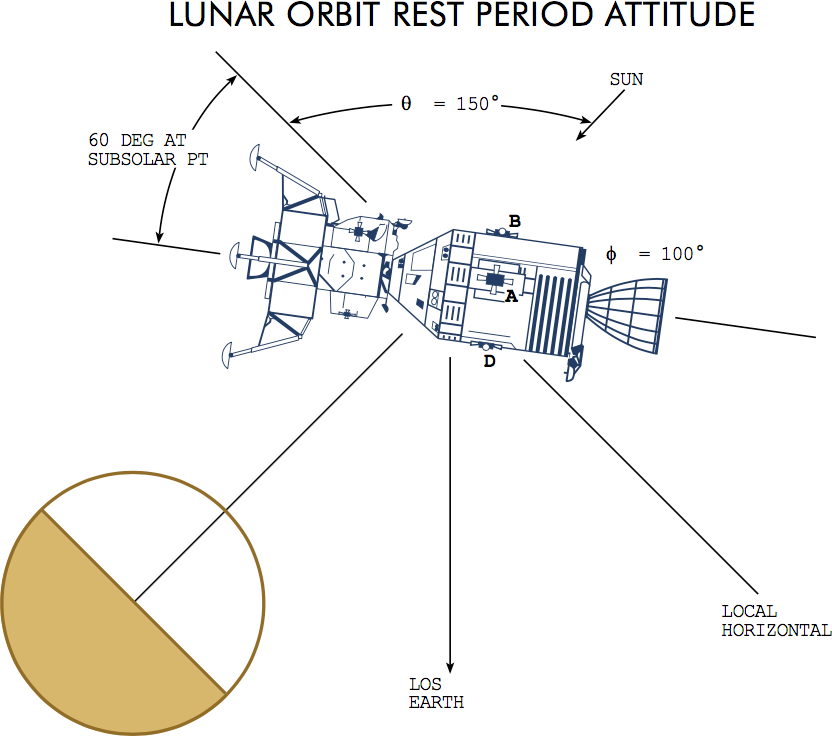
\includegraphics[width=\textwidth]{images/lunarorbitrestperiod.png}
    \end{figure}
    \vspace*{\fill}
\fi



\chapter[Friday]{Friday Events}

% This is true if only doing the flight manual, not the pre-flight
\ifisflight
\putchapterthumb
\fi


\vbox{
\subsection*{Morning Yoga }
\begin{description}[leftmargin=6em,noitemsep,style=nextline]
   \item[Location:] Acrodesiac Lunartics
    \item[Start time:] 9:00 AM
\end{description}

Gentle yoga flow, all levels. Come stretch and move in our beautiful, shaded studio! 

Bring a mat if you have one, if not, we have extras!
}

\vbox{
\subsection*{Multi-Sensory Meditation Experience ~ Mental Immersions}
\begin{description}[leftmargin=6em,noitemsep,style=nextline]
   \item[Location:] Axis Mundi
    \item[Time:] 9:30 AM -- 9:50 AM
\end{description}

Are you ready to go on a journey?
 Join Axis Mundi for an Immersive experience beyond earthly tethers. Our Master Meditation Instructor will lead you through a mental journey enhanced by beautiful digital visuals on our dome ceiling; as the rest of your senses are tantalized with aromatherapy, tactical sensations and audible bliss. 
 

We will provide essentials oils, digital visuals in our dome tent, music  etc..
}

\vbox{
\subsection*{Morning Yoga with Hard Left}
\begin{description}[leftmargin=6em,noitemsep,style=nextline]
   \item[Location:] Axis Mundi
    \item[Start time:] 10:00 AM
\end{description}

Axis Mundi will hold an All Levels Yoga session with Hard Left aka Yogini Merri. This vinyasa based morning practice is lead by a yogi Master with 2 decades of teaching experience. As we weave throughout the myofascial trains for the muscular system, we will unwind the mind and open our hearts to the energy that our burn community creates. Yoga mats and props will be provided. Enjoy our infused waters after class and mingle with the Gods and Goddesses of Axis Mundi. 

We will provide mats and props
}

\vbox{
\subsection*{Flow n Juice}
\begin{description}[leftmargin=6em,noitemsep,style=nextline]
   \item[Location:] Mermaid Oasis
    \item[Start time:] 10:00 AM
\end{description}

Yoga practice then drink fresh pressed juice 

Bring a Yoga mat 
}

\vbox{
\subsection*{Heart Chakra Kundalini}
\begin{description}[leftmargin=6em,noitemsep,style=nextline]
   \item[Location:] Moonspiracy
    \item[Start time:] 10:00 AM
\end{description}

This is short all-level kundalini practice that involves rapid breathing technique known as breath of fire. No prior experience is required. 

Mats and blocks are suggested but no materials are required.
}

\vbox{
\subsection*{Multi-Sensory Meditation Experience ~ Mental Immersions}
\begin{description}[leftmargin=6em,noitemsep,style=nextline]
   \item[Location:] Axis Mundi
    \item[Time:] 10:30 AM -- 10:50 AM
\end{description}

Are you ready to go on a journey?
 Join Axis Mundi for an Immersive experience beyond earthly tethers. Our Master Meditation Instructor will lead you through a mental journey enhanced by beautiful digital visuals on our dome ceiling; as the rest of your senses are tantalized with aromatherapy, tactical sensations and audible bliss. 
 

We will provide essentials oils, digital visuals in our dome tent, music etc..
}

\vbox{
\subsection*{Kundalini Yoga w/Siri Amrit}
\begin{description}[leftmargin=6em,noitemsep,style=nextline]
   \item[Location:] Miso Sexy
    \item[Host:] MerBuddah Triangle
    \item[Time:] 10:30 AM -- 11:30 AM
\end{description}

Yoga \& Meditation  

}

\vbox{
\subsection*{The Lunar Yearbook}
\begin{description}[leftmargin=6em,noitemsep,style=nextline]
   \item[Location:] See Art map!
    \item[Time:] 11:00 AM -- 2:00 PM
\end{description}

Making a highschool style yearbook and take peoples portraits for it 

}

\vbox{
\subsection*{Sensual four hand massage}
\begin{description}[leftmargin=6em,noitemsep,style=nextline]
   \item[Location:] Herhisensua
    \item[Time:] 11:00 AM -- 4:00 PM
\end{description}

Sensual massage 

}

\vbox{
\subsection*{Nude Model Figure Class}
\begin{description}[leftmargin=6em,noitemsep,style=nextline]
   \item[Location:] Martian Playground 
    \item[Host:] The Hive
    \item[Time:] 11:00 AM -- 1:00 PM
\end{description}

The Hive will be hosting a nude model figure drawing class. We will provide light refreshments, swag and deep shade during the hottest part of the day! 

We will provide all art supplies and materials. Just bring yourself and your creativity!
}

\vbox{
\subsection*{Tilted Hanger Dresses the Lunartics}
\begin{description}[leftmargin=6em,noitemsep,style=nextline]
   \item[Location:] The Tilted Hanger
    \item[Time:] 11:00 AM -- 4:00 PM
\end{description}

Tilted Hanger invites all (radical inclusion) to engage (participate) in (radical self expression) in finding your true burner self! We believe it is our duty (civic responsibility) to guide you in your freedom to receive without a price (de-commodified), receive without having to return (gifted) an experience from your community (communal effort), as we challenge you to become (self reliant) and to (leave no trace) ie. take your undies with you! (immediacy) 

All clothing provided, all you need to do is strut our runway in your new outfit!
}

\vbox{
\subsection*{Empathy vs. Sympathy avoiding karmic entanglements.}
\begin{description}[leftmargin=6em,noitemsep,style=nextline]
   \item[Location:] Axis Mundi
    \item[Start time:] 11:30 AM
\end{description}

Learn to use your energy and powers wisely. Learn what your magic is and how to use it without getting drained or over involved in situation that do not serve your evolution. Learn how to decipher intuition from triggers, love from attachment and connection from control. 

}

\vbox{
\subsection*{A Berry Delicious Time}
\begin{description}[leftmargin=6em,noitemsep,style=nextline]
   \item[Location:] Department of Synergy
    \item[Time:] 12:00 PM -- 2:00 PM
\end{description}

Come try out miracle berries!  They turn bitter tastes sweet, so lemons taste like lemonade, sour cream becomes yogurt, and sour IPAs and lambics become even more delicious beverages.  And Guinness becomes Irish chocolate milk!

We'll have lemons, limes, sour cream, apple vinegar, super sour candies, and other bitter delights.   These will miraculously transform to sweet, delicious goodness after coating your tongue with a tablet containing miraculin made from fruit of the "Miracle Berry" plant.

When life hands you lemons ... well, just try this because making lemonade is a PITA.

This is a kid friendly event!  (Barring the lambics and Guinness, of course!)  

}

\vbox{
\subsection*{Burner 101 ”learn to burn”}
\begin{description}[leftmargin=6em,noitemsep,style=nextline]
   \item[Location:] Launchpad
    \item[Host:] 2019 Greeters Team
    \item[Start time:] 12:00 PM
\end{description}

An interactive, fun, classroom style burner education system for burners new and old!! “Free tuition”  

}

\vbox{
\subsection*{Flogger making}
\begin{description}[leftmargin=6em,noitemsep,style=nextline]
   \item[Location:] Herhisensua/Red Cube
    \item[Time:] 1:00 PM -- 2:00 PM
\end{description}

Make your own flogger 

}

\vbox{
\subsection*{"Space Force Space-ic Training"}
\begin{description}[leftmargin=6em,noitemsep,style=nextline]
   \item[Location:] In front of Spontaneous Combustion. Can't miss it on the way to the BARge. 
    \item[Time:] 2:00 PM -- 5:00 PM
\end{description}

Greetings Hippies! We are Space Force: Moon Base. Do you want to see the galaxy? Can you make the Kessel Run in less than 12 parsecs? Are you romantically interested in green humanoids? If so, come find us by Spontaneous Combustion to see if you have what it takes to join our mission in spreading burner love and sweet, sweet democracy throughout the Milky Way. Come test your mettle in "Space-ic Training," a fun series of activities such as Space Blaster Marksmanship, Low Gravity Movement Drills, Lightsaber Combat, and Bubble Suit Sumo. Completion of these tasks will earn you some custom swag and entry into the Pugil Tournament and Free for All Laser Tag starting from 5 until Dark Thirty. At night (Thu-Sat), come back to complete your final training event: The Wormhole Simulator, a shiny, colorful art installation meant to test your resilience to the mind-altering effects of the Warp.  

All Materials will be provided. Bring your enthusiasm. 
}

\vbox{
\subsection*{Kundalini Yoga Meditation and Deep Relaxation Class"}
\begin{description}[leftmargin=6em,noitemsep,style=nextline]
   \item[Location:] Axis Mundi
    \item[Host:] Certified Kundalini teacher Sabrina Wells
    \item[Start time:] 2:30 PM
\end{description}

 Come awaken your kundalini serpent energy with warm up yoga exercises to loosen the spine, a short kriya and an extended meditation to uplift and elevate your conscious mind to prepare you for the rest of the weekend. Class will end with a long, deep relaxation and guided meditation. Yoga mat not necessary. 

}

\vbox{
\subsection*{AcroYoga Jam: Flying on the Moon }
\begin{description}[leftmargin=6em,noitemsep,style=nextline]
   \item[Location:] Acrodesiac Lunartics
    \item[Start time:] 3:00 PM
\end{description}

Come learn to fly on the moon...literally! Your Knoxville based AcroYoga community is excited to teach newbies and play with experienced AcroYoga Lunartics. We will have people from our camp there to base, spot and fly with you! We have an awesome yoga space / shade structure and plenty of mats. Don't be shy!  

We will provide mats and shade!
}

\vbox{
\subsection*{Hair braiding with Hippies}
\begin{description}[leftmargin=6em,noitemsep,style=nextline]
   \item[Location:] Hippie Haven
    \item[Time:] 3:00 PM -- 4:00 PM
\end{description}

We will be braiding each other’s hair! Come gift your braiding abilities, accessories, or just your fantastic energy and join us as we maintain our manes!  

This will be a daily event from 3-4 and run a little later as needed
}

\vbox{
\subsection*{The Pink Taco Hour!}
\begin{description}[leftmargin=6em,noitemsep,style=nextline]
   \item[Location:] The Hive
    \item[Time:] 3:00 PM -- 4:00 PM
\end{description}

Come visit The Hive at our camp from 3 PM to 4 PM for tacos and lavender lemonade! Soft shell tacos and lemonade will be served until we run out.

The Hive will also have a late night fire pit on Friday night and Saturday night until sunrise. Wanderers welcome! 

We will provide all delicious materials!
}

\vbox{
\subsection*{Consent to get Consent: An Intoxication and Consent Workshop}
\begin{description}[leftmargin=6em,noitemsep,style=nextline]
   \item[Location:] Martian Playground 
    \item[Time:] 4:00 PM -- 5:00 PM
\end{description}

Workshop: Practical harm reduction strategies for burning sexy when you don’t plan to be sober. An advanced conversation about the intersection of intoxication and consent. Telling you knuckleheads not to do it doesn't always work so let’s talk about it.  -- From Martian! 

}

\vbox{
\subsection*{Mad Tea Party}
\begin{description}[leftmargin=6em,noitemsep,style=nextline]
   \item[Location:] Holy Catrimony
    \item[Start time:] 5:00 PM
\end{description}

Join us at Holy Catrimony for a delightful array of teas, treats, and tricks. Bring a cup and sample the Tea Master's selections while our camp puts on a Wonderland variety show. Expect poetry recitation, musical performances, and at least one pocket watch full of butter (it is the best butter).  

We're providing snacks, tea, and entertainment
}


\ifisporto
\else
    \vspace*{\fill}
    \begin{figure}[!h]
    \centering
    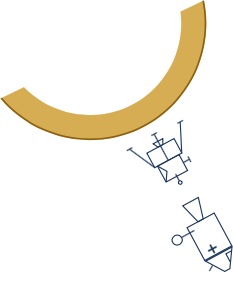
\includegraphics[width=.8\textwidth]{images/landing1.png}
    \end{figure}
\fi

\vbox{
\subsection*{"Space Force Space-ic Training"/Pugil Tournament and Free for All Laser Tag}
\begin{description}[leftmargin=6em,noitemsep,style=nextline]
   \item[Location:] In front of Spontaneous Combustion. Can't miss it on the way to the BARge. 
    \item[Time:] 5:00 PM -- 7:00 PM
\end{description}

Greetings Hippies! We are Space Force: Moon Base. Do you want to see the galaxy? Can you make the Kessel Run in less than 12 parsecs? Are you romantically interested in green humanoids? If so, come find us by Spontaneous Combustion to see if you have what it takes to join our mission in spreading burner love and sweet, sweet democracy throughout the Milky Way. Come test your mettle in "Space-ic Training," a fun series of activities such as Space Blaster Marksmanship, Low Gravity Movement Drills, Lightsaber Combat, and Bubble Suit Sumo. Completion of these tasks will earn you some custom swag and entry into the Pugil Tournament and Free for All Laser Tag starting from 5 until Dark Thirty. At night (Thu-Sat), come back to complete your final training event: The Wormhole Simulator, a shiny, colorful art installation meant to test your resilience to the mind-altering effects of the Warp.  

All Materials will be provided. Bring your enthusiasm. 
}

\vbox{
\subsection*{BDSM 101 - Negotiation, Consent, and Safety}
\begin{description}[leftmargin=6em,noitemsep,style=nextline]
   \item[Location:] Martian Playground 
    \item[Time:] 5:00 PM -- 6:00 PM
\end{description}

A panel of experienced kinky people discuss how to maintain informed and enthusiastic consent while playing with power exchange and sadomasochism. Any experience or interest level welcome! Bring your questions-this will be an open forum to share information. Time permitting, a live demo of putting someone into subspace and what consent looks like in that scenario will be included. 

}

\vbox{
\subsection*{Cock-Tails}
\begin{description}[leftmargin=6em,noitemsep,style=nextline]
   \item[Location:] Moonspiracy
    \item[Time:] 5:00 PM -- 7:00 PM
\end{description}

cock-tails: 5:00-7:00 at moonspiracy bar
we'll be serving up some brews and hard-on liqour drinks. Come by for a stiff one 
 

}

\vbox{
\subsection*{Create your prayer flag }
\begin{description}[leftmargin=6em,noitemsep,style=nextline]
   \item[Location:] Zentopia 
    \item[Host:] Banta
    \item[Time:] 5:00 PM -- 7:00 PM
\end{description}

Att: sinner-saints, manual praying isn't going to get it done, not with the baggage we're caring around. And fossil fuels are a horrible way to power your praying. Here's your chance to create a 100% breeze operated prayer flag. Every flap is guaranteed to carry your personalized message to one or more gods.

Bring costume, clothing, fabric, repairs and upgrades. 

}

\vbox{
\subsection*{Purple Pirate Party}
\begin{description}[leftmargin=6em,noitemsep,style=nextline]
   \item[Location:] Alcoholic Alliterators
    \item[Time:] 6:00 PM -- 8:00 PM
\end{description}

Is this where I put my description? 'Cause this is where it's gonna go.

Avast Ye! Pirates 'ave boarded the bar at Alcoholic Alliterators with plenty of the popular purple pirate potion to keep both land lubbers an' old salts alike afloat. Dress in yer favorite pirate regalia, bring yer jolly Roger, an' sing ship shanties with the cap'n an' crew! 
Ps. Bring yer cup! Huzzah! 

}

\vbox{
\subsection*{Kinky massage}
\begin{description}[leftmargin=6em,noitemsep,style=nextline]
   \item[Location:] Herhisensua
    \item[Time:] 6:00 PM -- 10:00 PM
\end{description}

Kinky massage 

}

\vbox{
\subsection*{Gerkins \& Merkins}
\begin{description}[leftmargin=6em,noitemsep,style=nextline]
   \item[Location:] Miso Sexy
    \item[Host:] MerBuddah Triangle
    \item[Start time:] 6:00 PM
\end{description}

Join us at Miso Sexy in the MerBuddah Triangle to explore our handmade fashion merkins \& enjoy some gerkins all in the name of word play, fermentation, \& keeping your naked bodies legal. How do you like your pickles? What is your dream merkin? Can't decide? It's no big dill! Come join the mermaids, throw back a pickle back, \& stick around for the Twerkshop to follow. 

We will provide Gerkin, Merkins \& pickle backs. Feel feel to bring any brines, whiskey, or merkins you'd like to share. 
}

\vbox{
\subsection*{Twerkshop}
\begin{description}[leftmargin=6em,noitemsep,style=nextline]
   \item[Location:] Miso Sexy
    \item[Time:] 6:00 PM -- 7:00 PM
\end{description}

Evolution of the twerk/find your rhythm and tap into your divine feminine 

}

\vbox{
\subsection*{The Hoooplah! }
\begin{description}[leftmargin=6em,noitemsep,style=nextline]
   \item[Location:] The Bermuda Pyramid
    \item[Host:] Andi Glytch
    \item[Time:] 6:00 PM -- 8:00 PM
\end{description}

Hooplah skill share time!! Beginners hoop and fan instruction can be given!! Open space and close enough to Headroom to hear some good music while we flow <3  

You will need to bring your own props!! I may have a few extra but not more than a few ;)  if absolutely without props, I would let you borrow mine <3 
}

\vbox{
\subsection*{Cuddle Concent}
\begin{description}[leftmargin=6em,noitemsep,style=nextline]
   \item[Location:] Zentopia 
    \item[Host:] Arelis
    \item[Start time:] 7:30 PM
\end{description}

Cuddling is a away we can deepen our connection to another and a away to heal our hearts. All genders and orintations welcomed.This class will demonstrate cuddling techniques while creating a space to continue the conversation around concent. Single and couples welcomed. 

}

\vbox{
\subsection*{The bourbon baked bean bash }
\begin{description}[leftmargin=6em,noitemsep,style=nextline]
   \item[Location:] Alcoholic Alliterators 
    \item[Time:] 8:00 PM -- 9:00 PM
\end{description}

Fun and wacky 

}

\vbox{
\subsection*{Space Bar}
\begin{description}[leftmargin=6em,noitemsep,style=nextline]
   \item[Location:] Department of Synergy
    \item[Time:] 8:00 PM -- 2:00 AM
\end{description}

From home brews with whimsical sciency names to fluorescent glowing drinks, enjoy some drinks at the Space Bar. 

}

\vbox{
\subsection*{Hippie Haven Presents:  LUNAR LAVA SANDWWHICHES}
\begin{description}[leftmargin=6em,noitemsep,style=nextline]
   \item[Location:] Hippie Haven
    \item[Start time:] 9:00 PM
\end{description}

Come make editable and burnable art! Our take on Smores is an interstellar masterpiece for your taste buds!   

All foods will be provided, but always feel free to donate or BYO.
}

\vbox{
\subsection*{Black Light Body Paint Acro }
\begin{description}[leftmargin=6em,noitemsep,style=nextline]
   \item[Location:] Acrodesiac Lunartics
    \item[Start time:] 10:00 PM
\end{description}

Acrodesiac Lunartics' Magical Yoga Space will be transformed into a black light celestial paradise! Become a canvas for black light body paint and then flow, dance, and fly creating colorful shapes! There will be plenty of feet to fly on so don't be shy! Hoops and other flow arts welcome. Event co-hosted by Herhisensua, who will be providing chill music.  

Black light body paint and mats provided
}


\ifisporto
\else
    \vspace*{\fill}
    \begin{figure}[!h]
    \centering
    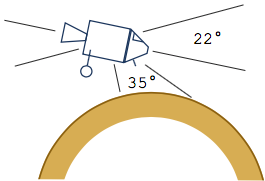
\includegraphics[width=.8\textwidth]{images/landing3.png}
    \end{figure}
    \vspace*{\fill}
    \begin{figure}[!h]
    \centering
    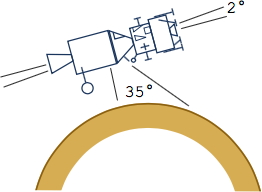
\includegraphics[width=.8\textwidth]{images/landing4.png}
    \end{figure}
    \vspace*{\fill}
\fi

\chapter[Saturday]{Saturday Events}

% This is true if only doing the flight manual, not the pre-flight
\ifisflight
\putchapterthumb
\fi

\vbox{
\subsection*{Be Your Burn}
\begin{description}[leftmargin=6em,noitemsep,style=nextline]
   \item[Location:] Miso Sexy
    \item[Start time:] 7:00 AM
\end{description}

Yoga/Meditation/Intention Setting 

}

\vbox{
\subsection*{Morning Yoga }
\begin{description}[leftmargin=6em,noitemsep,style=nextline]
   \item[Location:] Acrodesiac Lunartics
    \item[Start time:] 9:00 AM
\end{description}

Gentle yoga flow, all levels. Come stretch and move in our beautiful, shaded studio space! 

Bring a mat if you have one, if not, we have extras!
}

\vbox{
\subsection*{Morning Yoga with Hard Left}
\begin{description}[leftmargin=6em,noitemsep,style=nextline]
   \item[Location:] Axis Mundi
    \item[Start time:] 10:00 AM
\end{description}

Axis Mundi will hold an All Levels Yoga session with Hard Left aka Yogini Merri. This vinyasa based morning practice is lead by a yogi Master with 2 decades of teaching experience. As we weave throughout the myofascial trains for the muscular system, we will unwind the mind and open our hearts to the energy that our burn community creates. Yoga mats and props will be provided. Enjoy our infused waters after class and mingle with the Gods and Goddesses of Axis Mundi. 

We will provide mats and props
}

\vbox{
\subsection*{Freeform radicaly inclusice energetic new dance (F.R.I.E.N.D)  skillshare}
\begin{description}[leftmargin=6em,noitemsep,style=nextline]
   \item[Location:] Martian Playground 
    \item[Host:] Coreythrowsthings
    \item[Time:] 10:30 AM -- 12:00 PM
\end{description}

Open skillshare to learn new flow arts, dance, prop manipulation. Bring your props and extra if you have them. let's all learn something new , and get burn day started right. 

I'll have a few extra props. But please bring your own and any you don't mind sharing!
}

\vbox{
\subsection*{Qi Gong}
\begin{description}[leftmargin=6em,noitemsep,style=nextline]
   \item[Location:] Miso Sexy
    \item[Host:] MerBuddah Triangle
    \item[Start time:] 10:30 AM
\end{description}

Qi Gong assists the free flow of energy through the channels of the body. It is generally practiced standing up so just bring yourself. Class will last about an hour and will take place in our shaded dome space. All levels welcome. 

}

\vbox{
\subsection*{The Lunar Yearbook}
\begin{description}[leftmargin=6em,noitemsep,style=nextline]
   \item[Location:] (not sure yet?) still waiting on placement
    \item[Time:] 11:00 AM -- 2:00 PM
\end{description}

Making a highschool style yearbook and take peoples portraits for it 

}

\vbox{
\subsection*{Sensual four hand massage}
\begin{description}[leftmargin=6em,noitemsep,style=nextline]
   \item[Location:] Herhisensua
    \item[Time:] 11:00 AM -- 4:00 PM
\end{description}

Sensual massage 

}

\vbox{
\subsection*{BAR[ge] Open Hours}
\begin{description}[leftmargin=6em,noitemsep,style=nextline]
   \item[Location:] In the middle of the river, can't miss it! 
    \item[Time:] 11:00 AM -- 7:00 PM
\end{description}

Come get refreshed on the BAR[ge]! H-F-S 11A - 7P. Daily drink specials (bring ID), ice cold water, and other non-alcoholic refreshments.  

Bring a cup.
}

\vbox{
\subsection*{Tilted Hanger Dresses the Lunartics}
\begin{description}[leftmargin=6em,noitemsep,style=nextline]
   \item[Location:] The Tilted Hanger
    \item[Time:] 11:00 AM -- 4:00 PM
\end{description}

Tilted Hanger invites all (radical inclusion) to engage (participate) in (radical self expression) in finding your true burner self! We believe it is our duty (civic responsibility) to guide you in your freedom to receive without a price (de-commodified), receive without having to return (gifted) an experience from your community (communal effort), as we challenge you to become (self reliant) and to (leave no trace) ie. take your undies with you! (immediacy) 

All clothing provided, all you need to do is strut our runway in your new outfit!
}

\vbox{
\subsection*{Shove a tennis ball up under your butt}
\begin{description}[leftmargin=6em,noitemsep,style=nextline]
   \item[Location:] Alcoholic Alliterators
    \item[Host:] Ocelot
    \item[Time:] 11:00 AM -- 5:00 PM
\end{description}

Have you ever felt the endorphin rush from a tennis ball up the ass? Well I can't help with that (needs a flared base), but you CAN use it to release your tight glutes! It'll feel pretty bad then really good. Come give it a try! Balls benefit sore shoulders, tight tushies, and cramped calves. 

Yes, I have the tennis balls
}

\vbox{
\subsection*{Sciencing the \faTrash\xspace Out of Your \faFire}
\begin{description}[leftmargin=6em,noitemsep,style=nextline]
   \item[Location:] Department of Synergy
    \item[Time:] 12:00 PM -- 2:00 PM
\end{description}

Come learn how the sun makes rainbows, how to power your alarm clock with a potato or a pickle, and how to make your own invisible ink. See the scales on a butterfly's wing, the fuzz on a bumble bee, and the hundreds of tiny flowers hidden in a daisy. Make a sun print, and pick out a small fossil to take home as a reminder of your visit to our Traveling Science Roadshow!

This is a kid friendly event! 

}

\vbox{
\subsection*{Burner 101 ”learn to burn”}
\begin{description}[leftmargin=6em,noitemsep,style=nextline]
   \item[Location:] Launchpad
    \item[Host:] 2019 Greeters Team
    \item[Start time:] 12:00 PM
\end{description}

An interactive, fun, classroom style burner education system for burners new and old!! “Free tuition”  

}


\ifisporto
\else
    \vspace*{\fill}
    \begin{figure}[!h]
    \centering
    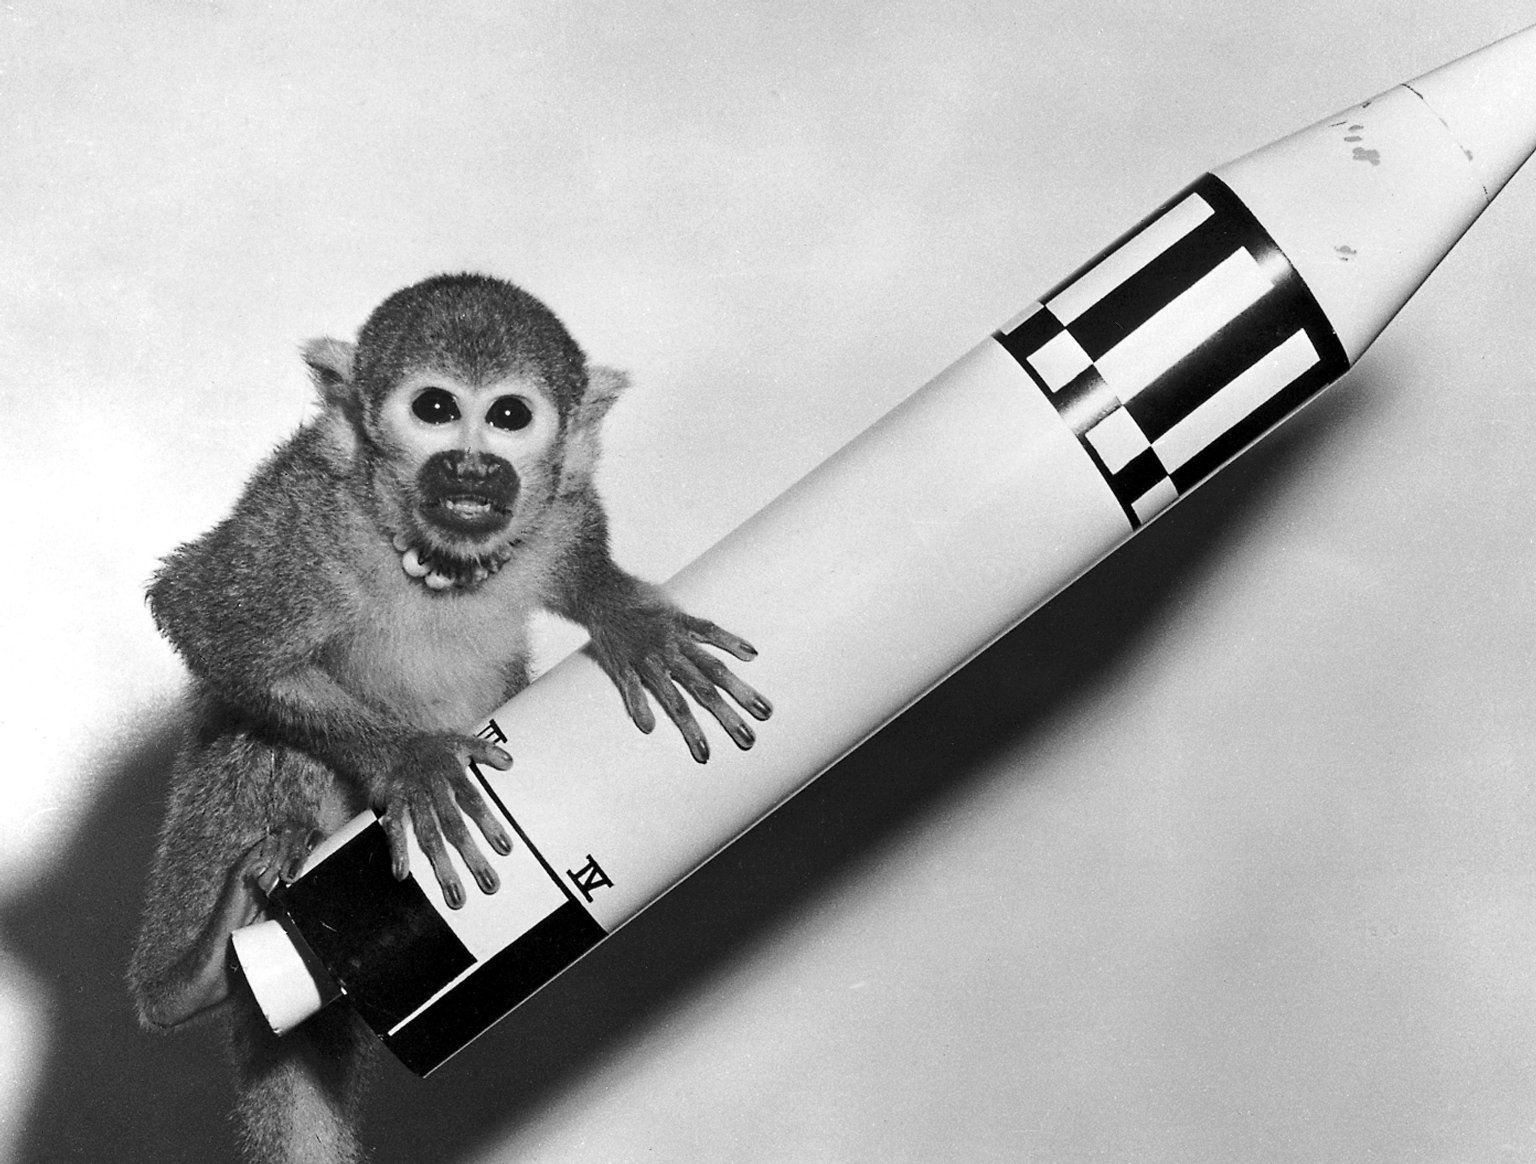
\includegraphics[width=\textwidth]{images/Baker.jpg}
    \end{figure}
    \vspace*{\fill}
\fi

\vbox{
\subsection*{Consciousness Ascension \& Soul Tribes: Taking Action and Making Connections}
\begin{description}[leftmargin=6em,noitemsep,style=nextline]
   \item[Location:] Martian Playground 
    \item[Host:] Rhythm Sin Mews
    \item[Start time:] 12:00 PM
\end{description}

Greetings fellow extraterrestrials, I am Rhythm Sin, a Divine Feminine Lemurian and Arcturian from Mintakan. This round-table and meetup is being held for the purpose of establishing roots or paths, and building soul tribes in order to work towards ascending the consciousness of the entirety of humankind. Topics will be directed by those in attendance (ie, bring your knowledge and content of interest) and include astrology, soul connections, healers, oracles/psychics, sacred plant/psychedelic medicine, the 13-month calendar, the first through twelfth chakras, Starseed/planetary origins, Lemuria and Atlantis, suppressed history and Egyptian spirituality. By working within the 4th dimension together we can vibrate the frequency of pure unconditional love into ourselves and resonate among others, and therefore bring 5th dimensional energies and the New Earth into integration with our current 3rd dimensional reality, propelling us into a collective consciousness state beyond our current abilities to imagine. 

}

\vbox{
\subsection*{Disco Brunch}
\begin{description}[leftmargin=6em,noitemsep,style=nextline]
   \item[Location:] Moonspiracy
    \item[Start time:] 12:00 PM
\end{description}

A yearly tradition since Alchemy many moons ago, Disco Brunch returns for another epic daytime event. Sexy disco jams and mimosas will be served aboard the struggle.  

Champagne and juice will be provided
}

\vbox{
\subsection*{Mummification}
\begin{description}[leftmargin=6em,noitemsep,style=nextline]
   \item[Location:] Herhisensua/Red Cube
    \item[Time:] 1:00 PM -- 2:00 PM
\end{description}

Mummification as bondage 

}

\vbox{
\subsection*{Nude Model Figure Class}
\begin{description}[leftmargin=6em,noitemsep,style=nextline]
   \item[Location:] Martian Playground 
    \item[Host:] The Hive
    \item[Time:] 1:00 PM -- 5:00 PM
\end{description}

The Hive will be hosting a nude model figure drawing class at Martian Playground. We will provide light refreshments, swag and deep shade during the hottest part of the day! 

We will provide all art supplies and materials. Just bring yourself and your creativity!
}

\vbox{
\subsection*{AcroYoga Jam: Flying on the Moon }
\begin{description}[leftmargin=6em,noitemsep,style=nextline]
   \item[Location:] Acrodesiac Lunartics
    \item[Start time:] 3:00 PM
\end{description}

Come learn to fly on the moon...literally! Your Knoxville based AcroYoga community is excited to teach newbies and play with experienced AcroYoga Lunartics. We will have people from our camp there to base, spot and fly with you! We have an awesome yoga space / shade structure and plenty of mats. Don't be shy!  

We will provide mats and shade!
}

\vbox{
\subsection*{Show us yours, We'll show you ours}
\begin{description}[leftmargin=6em,noitemsep,style=nextline]
   \item[Location:] Herhisensua/Red Cube
    \item[Time:] 3:00 PM -- 4:00 PM
\end{description}

Show us and tell us about your favorite kinky toys 

}

\vbox{
\subsection*{The Pink Taco Hour!}
\begin{description}[leftmargin=6em,noitemsep,style=nextline]
   \item[Location:] The Hive
    \item[Time:] 3:00 PM -- 4:00 PM
\end{description}

Come visit The Hive at our camp from 3 PM to 4 PM for tacos and lavender lemonade! Soft shell tacos and lemonade will be served until we run out.

The Hive will also have a late night fire pit at our camp on Friday night and Saturday night until sunrise. Wanderers welcome!  

We will provide all delicious materials!
}

\vbox{
\subsection*{Mermaid Parade}
\begin{description}[leftmargin=6em,noitemsep,style=nextline]
   \item[Location:] Mermaid Oasis
    \item[Start time:] 3:30 PM
\end{description}

All are invited to parade around the burn as Merfolk and creatures of the sea spreading hydration from our Jellyfish Hydration Station cart, spreading a wave of MERiment and Sexy Moisture to everyone who swims in nearby currents!

Don't have sea attire?  Come to the Mermaid Oasis  before the start of the parade and we will adorn you or join with us on our wave.  

}

\vbox{
\subsection*{Tan n Tasty}
\begin{description}[leftmargin=6em,noitemsep,style=nextline]
   \item[Location:] Moonspiracy
    \item[Time:] 5:00 PM -- 7:00 PM
\end{description}

Tan n Tasty: come by moonspiracy bar for tasty drinks made by tan ladies in pasties! 
feat. liquid marijuanas, black n tans, and many more tropical tonics, drafts, and libations 
 

}

\vbox{
\subsection*{Create your prayer flag }
\begin{description}[leftmargin=6em,noitemsep,style=nextline]
   \item[Location:] Zentopia 
    \item[Host:] Banta
    \item[Time:] 5:00 PM -- 7:00 PM
\end{description}

Att: sinner-saints, manual praying isn't going to get it done, not with the baggage we're caring around. And fossil fuels are a horrible way to power your praying. Here's your chance to create a 100% breeze operated prayer flag. Every flap is guaranteed to carry your personalized message to one or more gods. 

}

\vbox{
\subsection*{I like}
\begin{description}[leftmargin=6em,noitemsep,style=nextline]
   \item[Location:] Part of Little Bohemia
    \item[Time:] 7:00 PM -- open ended
\end{description}

tie dye 

Bring your own clothes or whatever only small items.
}

\vbox{
\subsection*{Michelle MaBelle's Pop Up Karaoke}
\begin{description}[leftmargin=6em,noitemsep,style=nextline]
   \item[Location:] Department of Synergy
    \item[Host:] Michelle MaBelle
    \item[Time:] 8:00 PM -- 2:00 AM
\end{description}

Come sing your heart out to your favorite songs! Serenade your campmates! Let your inner rockstar out in a fit of radical self expression! (No mic drops, though, please!) 

}

\vbox{
\subsection*{Multi-Sensory Meditation Experience ~ Mental Immersions}
\begin{description}[leftmargin=6em,noitemsep,style=nextline]
   \item[Location:] Axis Mundi
    \item[Start time:] 10:00 PM
\end{description}

Are you ready to go on a journey?
 Join Axis Mundi for an Immersive experience beyond earthly tethers. Our Master Meditation Instructor will lead you through a mental journey enhanced by beautiful digital visuals on our dome ceiling; as the rest of your senses are tantalized with aromatherapy, tactical sensations and audible bliss. 
 

}


\ifisporto
\else
    \vspace*{\fill}
    \begin{figure}[!h]
    \centering
    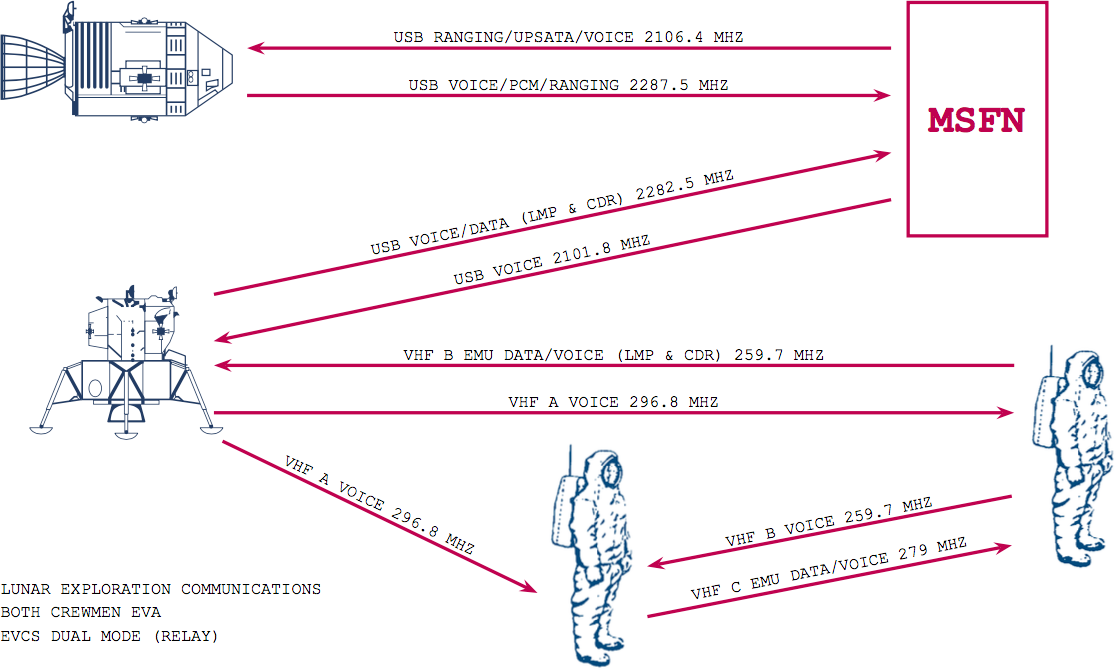
\includegraphics[width=\textwidth]{images/communication1.png}
    \end{figure}
    \vspace*{\fill}
\fi


\chapter[Sunday]{Sunday Events}

% This is true if only doing the flight manual, not the pre-flight
\ifisflight
\putchapterthumb
\fi

\vbox{
\subsection*{Morning Yoga }
\begin{description}[leftmargin=6em,noitemsep,style=nextline]
   \item[Location:] Acrodesiac Lunartics
    \item[Start time:] 9:00 AM
\end{description}

Gentle yoga flow, all levels. Come stretch and move in our beautiful, shaded studio! 

Bring a mat if you have one, if not, we have extras!
}

\vbox{
\subsection*{Walking Meditation with Sam}
\begin{description}[leftmargin=6em,noitemsep,style=nextline]
   \item[Location:] Acrodesiac Lunartics
    \item[Start time:] 10:00 AM
\end{description}

A guided walking mediation, lead by Sam. Following our morning yoga practice.  

}

\vbox{
\subsection*{Sunbathing Yin Yoga}
\begin{description}[leftmargin=6em,noitemsep,style=nextline]
   \item[Location:] Mermaid Oasis
    \item[Start time:] 10:00 AM
\end{description}

Yin Yoga in the sunshine 

Bring a Yoga mat
}

\vbox{
\subsection*{Elevated Arrogant Sunday Smoothies}
\begin{description}[leftmargin=6em,noitemsep,style=nextline]
   \item[Location:] Moonspiracy/Headroom Bar 
    \item[Start time:] 10:00 AM
\end{description}

Headroom will be serving up Smooth Tunes and Smoothies to energize the hippies with nutrients, fruit and fun!  

}

\vbox{
\subsection*{The Lunar Yearbook}
\begin{description}[leftmargin=6em,noitemsep,style=nextline]
   \item[Location:] See Art map at the end of the Pocket Guide!
    \item[Time:] 11:00 AM -- 2:00 PM
\end{description}

Making a highschool style yearbook and take peoples portraits for it 

}

\ifisporto
\else
    \newpage
\fi

\vbox{
\subsection*{AcroYoga Jam: Flying on the Moon }
\begin{description}[leftmargin=6em,noitemsep,style=nextline]
   \item[Location:] Acrodesiac Lunartics
    \item[Start time:] 1:00 PM
\end{description}

Come learn to fly on the moon...literally! Your Knoxville based AcroYoga community is excited to teach newbies and play with experienced AcroYoga Lunartics. We will have people from our camp there to base, spot and fly with you! We have an awesome yoga space / shade structure and plenty of mats. Don't be shy!  

We will provide mats and shade!
}

\vbox{
\subsection*{The Many Methods to MA. ke Your Own Gem Elixir }
\begin{description}[leftmargin=6em,noitemsep,style=nextline]
   \item[Location:] Mermaid Oasis
    \item[Host:] Amazonite
    \item[Time:] 3:33 PM -- 4:44 PM
\end{description}

Gather at the Mermaid Oasis to learn how to utilize and create gem elixirs. We will have crystal grid templates to play with so each participant can infuse a healing intention into water. Bring your own favorite crystals, or use ours, to capture the inspiration and healing of the moon and take it with you for use in defaultia. Bring a small jar, spray bottle, or tincture bottle if you are able, we will have a few to gift.  

Water, crystals, and vodka (to preserve your elixir) will be provided for making the elixir. A few tincture bottles/small jars/spray bottles will be available but participants are encouraged to bring their own.  
}

% \section*{Thursday-Saturday}



% \vspace*{\fill}
% \begin{center}
% 	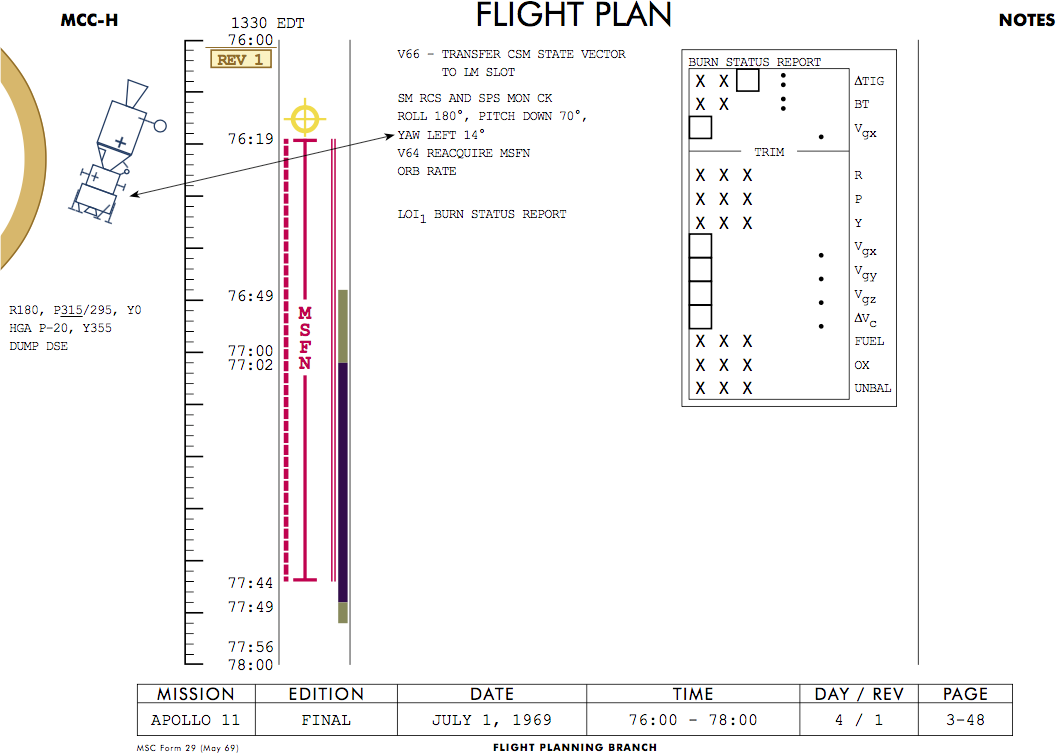
\includegraphics[width=.8\textwidth]{images/flightplan2}
% \end{center}
% \vspace*{\fill}

% \newpage
% \pagestyle{empty}
% \vspace*{\fill}
% \begin{center}
% \texttt{THIS PAGE INTENTONALLY LEFT BLANK.}
% \end{center}
% \vspace*{\fill}


